% ==================================================
% Accumulator Data Structure
% Author: Lester James V. Miranda
% ==================================================

\documentclass[preview, convert={outfile=\jobname.png,density=300}]{standalone}

\usepackage{tikz}
\usepackage{color}
\usepackage{subfig}
\usepackage{ifthen}

\renewcommand\familydefault{\sfdefault}

\usetikzlibrary{
    matrix,
    shapes,
    fit,
    arrows.meta,
    arrows,
    positioning,
    calc,
    backgrounds,
    shadows.blur,
    shapes.geometric,
}

\begin{document}
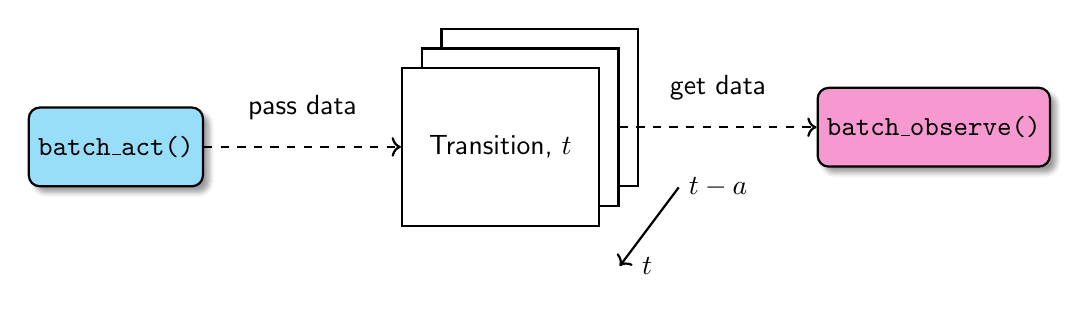
\begin{tikzpicture}[
    node distance= 1cm and 2.5cm,
    call/.style={draw, thick, rounded corners, text=black, align=center,
                minimum width=2cm,minimum height=1cm,fill=white, 
                blur shadow={shadow blur steps=5}},
    file/.style={draw, thick, fill=white, minimum width=2.5cm, minimum height=2cm},
    textbox/.style={fill=none, align=center, minimum height=0.7cm, minimum width=0.7cm},
]

\node[file] at (0,0) (rear) {};
\node[file] at (-0.25,-0.25) (mid) {};
\node[file] at (-0.50,-0.50) (front) {Transition, $t$};

\node[call, fill=cyan!40] (batchAct) [left=of front] {\texttt{batch\_act()}}; 
\draw[->, dashed, thick] (batchAct) -- (front) node[midway, yshift=0.5cm] {pass data};

\node[call, fill=magenta!40] (batchObserve) [right=of mid] {\texttt{batch\_observe()}}; 
\draw[->, dashed, thick] (mid) -- (batchObserve) node[midway, yshift=0.5cm] {get data};

\draw[->, thick] ([xshift=0.5cm]rear.south east) -- ([xshift=0.25cm,yshift=-0.5cm]front.south east);

\node[textbox] at ([xshift=1cm]rear.south east) {$t-a$};
\node[textbox] at ([xshift=0.6cm,yshift=-0.5cm]front.south east) {$t$};


\end{tikzpicture}
\end{document}
